%This is the base for the certificat of the chatoische catalysator stipendien

\documentclass{article}
\title{Chaotisches Catalysator Stipendium}
%\date{2022/2023}
%\name{Mars Mustermensch}

%Packages used:
\usepackage{graphicx}
\usepackage[T1]{fontenc}
\usepackage{fontspec} % used to set custom font
\usepackage[a4paper, margin=0.5cm]{geometry}
\usepackage[document]{ragged2e}
\usepackage{changepage}
\usepackage{tikz} %used to place text over images
\usepackage{subfig}

%removes page number
\pagenumbering{gobble}

% Setting font sizes:
\newcommand{\smallfont}[1]{{%
  \fontsize{13pt}{16pt}\normalfont #1%
}}
\newcommand{\normfont}[1]{{%
  \fontsize{20pt}{24pt}\normalfont #1%
}}
\newcommand{\bigfont}[1]{{%
  \fontsize{30pt}{36pt}\normalfont #1%
}}

% Setting custom fonts:
\newfontfamily{\firasans}
  [Ligatures=TeX, % recommended
   UprightFont={*-Light},
   ItalicFont={*-Italic},
   BoldFont={*-Medium}]
  {FiraSans}
\newfontfamily{\monomaniac}
  [Ligatures=TeX, % recommended
  ]
  {MonomaniacOne-Regular.ttf}

%--------------------------------------------------------------------------------------------

\begin{document}

\begin{tikzpicture}
    \draw (0, 0) node[inner sep=0] {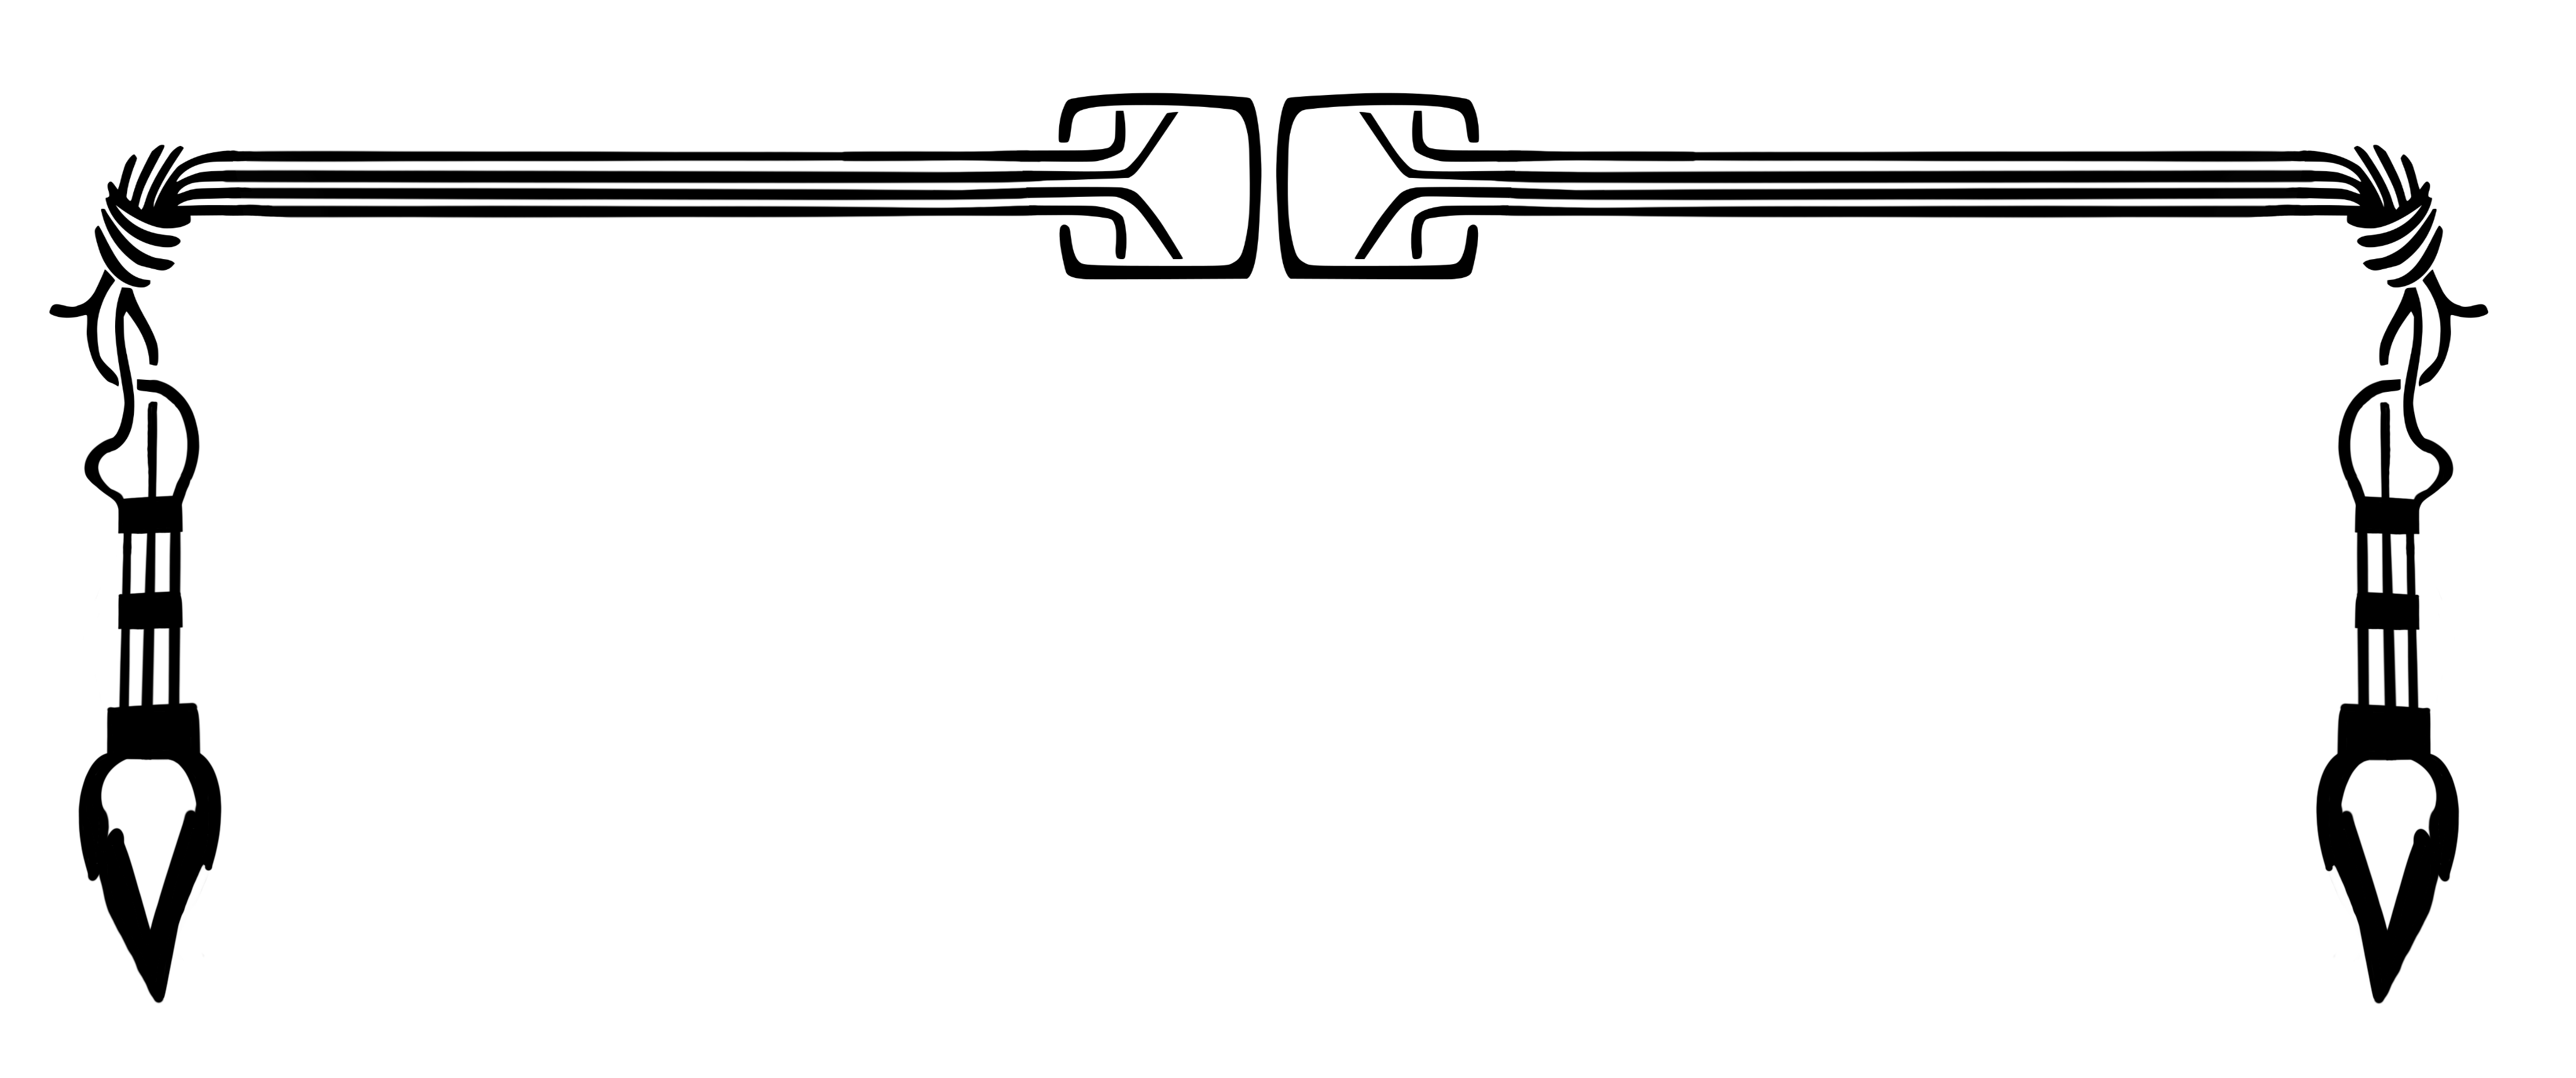
\includegraphics[width=0.97\paperwidth]{header}};
    \draw (0, 0) node {\normfont{\monomaniac 2023}};
    \draw (0, -1) node {\bigfont{\monomaniac Chaotisches Catalysator}};
    \draw (0, -2) node {\bigfont{\monomaniac Stipendium}};
    \draw (0, -3) node {\normfont{\monomaniac - Mars Mustermensch -}};
\end{tikzpicture}

\vspace{0.9cm}

\begin{adjustwidth}{3cm}{3cm}
    \smallfont{\firasans \RaggedRight  \\ \smallskip
    Moin Mars Mustermensch, \bigskip
    
    Wir freuen uns, dir im Namen des Chaos Computer Clubs mitteilen zu können, dass du ein Chaotischen Catalysator Stipendium erhalten hast! \\ \bigskip
    Auf der Suche nach Arbeiten, welche die Welt zu einem besseren Ort machen und die Grundätze der Hacker*innen Ethik aufgreifen, hast du uns mit deiner Idee überzeugt. \\
    Aus diesem Grund fördern wird dich mit 1.500€ und begrüßen dich stolz im Kreis der Stipendiat*innen.\\ \bigskip

    Es freut uns, diesen bedeutenden Meilenstein mit dir zu feiern, und wir freuen uns darauf Zeug*innen deines weiteren Erfolgs zu werden, die Welt durch deinen  Beitrag zu Technologie und Forschung zu bereichern. \\ 
    Nun liegt es an dir Mehrwert zu schaffen. Wir glauben an dich. \\ \bigskip
    
    
    Herzlichen Glückwunsch und alles Gute für die Zukunft!\\[3\baselineskip]
    \par}
\end{adjustwidth}

\begin{adjustwidth}{3cm}{3cm}
    \RaggedLeft ---------------------------------------- \\
    \smallfont{\firasans Samuel Brinkmann}
\end{adjustwidth}

\begin{figure}[b]
	\begin{center}
		
\includegraphics[width=0.9\paperwidth] {deco_bottom}
	\end{center}
\end{figure}

\end{document}